% \section{Router API}
\section{Router API}

% The exported API of the Angular Router package can be represented as:

Angular Router 包导出的 API 结构\fref{fig:router_api_1}、\ref{fig:router_api_2} 和 \ref{fig:router_api_3}。

\begin{figure}[!hbt]
  \centering
  \caption{Angular Router API (part 1)}
  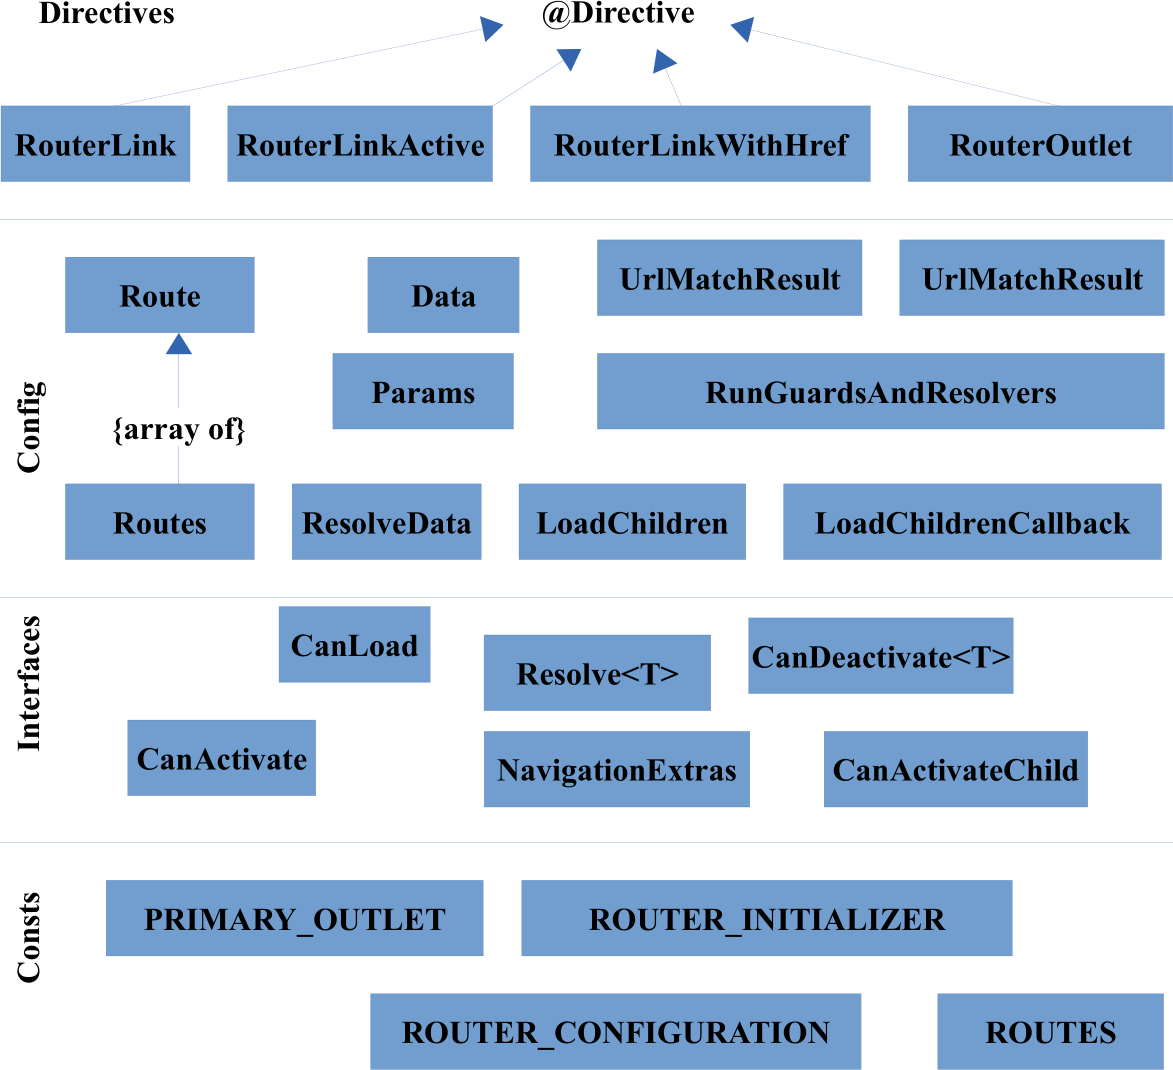
\includegraphics[width=0.55\linewidth]{13_the_router_package/router_api_1}
  \label{fig:router_api_1}
\end{figure}

\begin{figure}[!hbt]
  \centering
  \caption{Angular Router API (part 2)}
  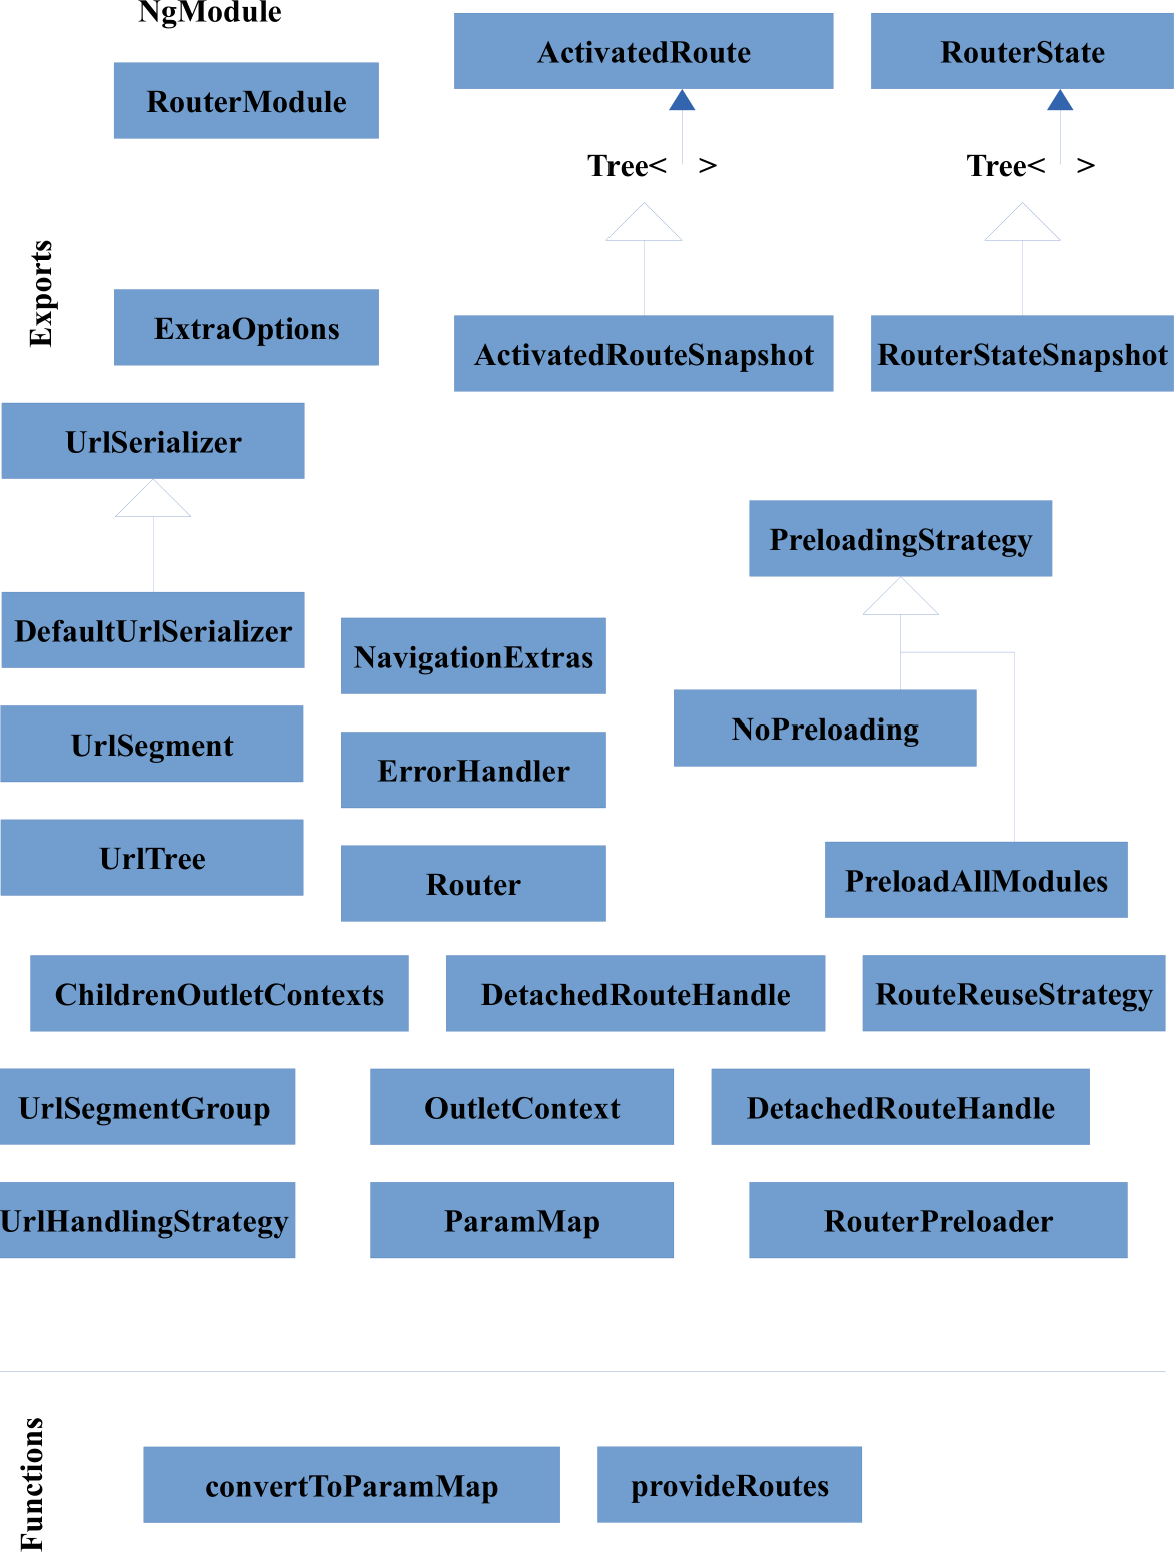
\includegraphics[width=0.75\linewidth]{13_the_router_package/router_api_2}
  \label{fig:router_api_2}
\end{figure}

\clearpage

\begin{figure}[!hbt]
  \centering
  \caption{Angular Router API (part 2)}
  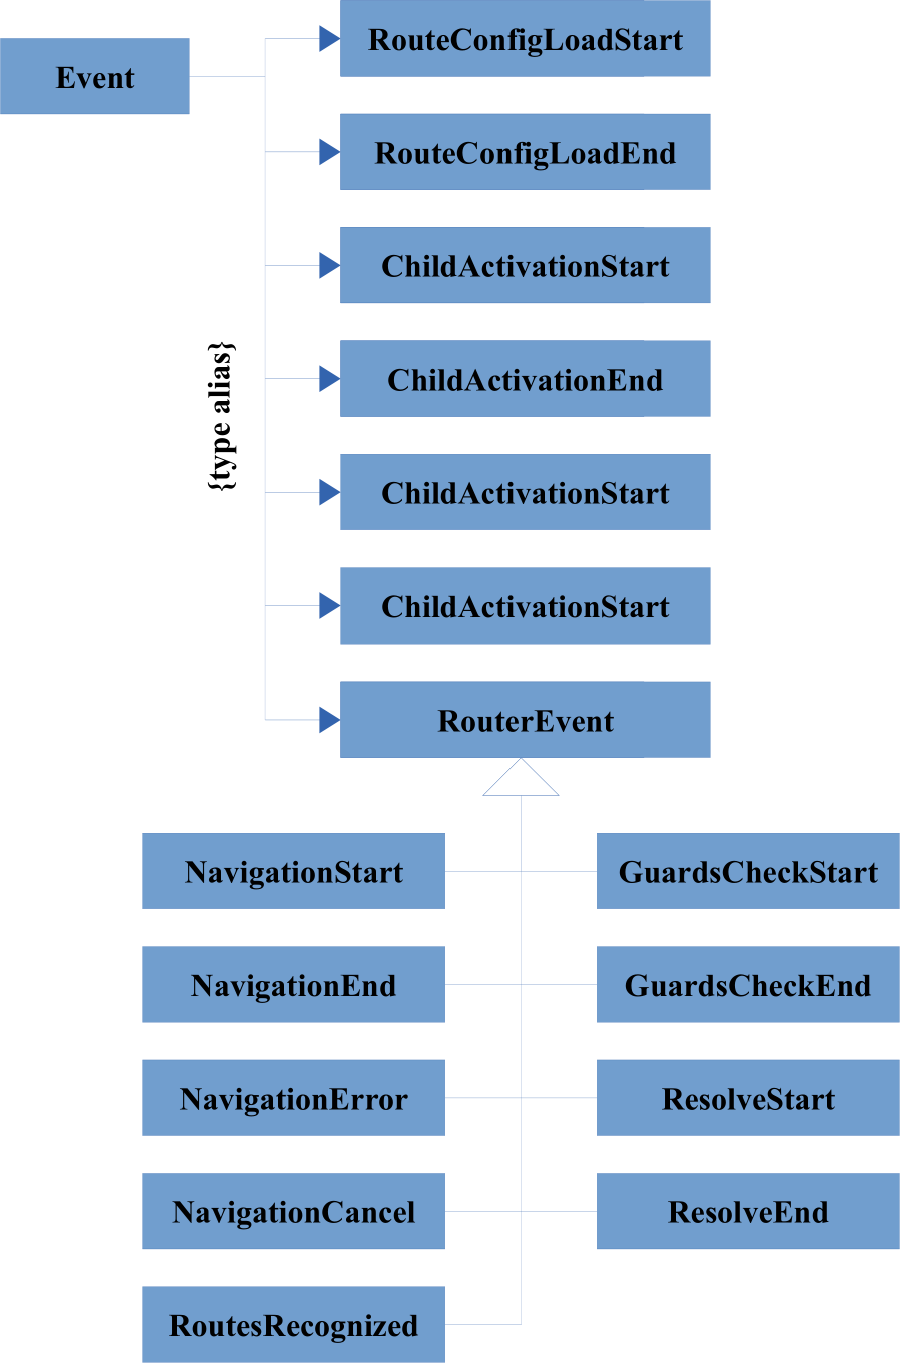
\includegraphics[width=0.75\linewidth]{13_the_router_package/router_api_3}
  \label{fig:router_api_3}
\end{figure}

\clearpage

% The Angular Router source tree is at:

Angular Router 源码位于:

\begin{itemize}
  \item \href{https://github.com/angular/angular/tree/master/packages/router}
        {<ANGULAR-MASTER>/packages/router}
\end{itemize}

% Its root directory contains index.ts, which just exports the contents of public\_api.ts,
% which in turn exports the contents of .src/index.ts.

根目录包含 index.ts,它只是导出了 public\_api.t 的内容,
而后者又导出\, .src/index.ts 的内容。

% This lists the exports and gives an initial impression of the size of the router package:

这列出了 exports 内容并给出了路由器包大小的初步印象:

\begin{minted}{typescript}
export {
  Data,
  LoadChildren,
  LoadChildrenCallback,
  ResolveData,
  Route,
  Routes,
  RunGuardsAndResolvers,
  UrlMatchResult,
  UrlMatcher,
} from './config';
export { RouterLink, RouterLinkWithHref } from './directives/router_link';
export { RouterLinkActive } from './directives/router_link_active';
export { RouterOutlet } from './directives/router_outlet';
export {
  ActivationEnd,
  ActivationStart,
  ChildActivationEnd,
  ChildActivationStart,
  Event,
  GuardsCheckEnd,
  GuardsCheckStart,
  NavigationCancel,
  NavigationEnd,
  NavigationError,
  NavigationStart,
  ResolveEnd,
  ResolveStart,
  RouteConfigLoadEnd,
  RouteConfigLoadStart,
  RouterEvent,
  RoutesRecognized,
} from './events';
export {
  CanActivate,
  CanActivateChild,
  CanDeactivate,
  CanLoad,
  Resolve,
} from './interfaces';
export {
  DetachedRouteHandle,
  RouteReuseStrategy,
} from './route_reuse_strategy';
export { NavigationExtras, Router } from './router';
export { ROUTES } from './router_config_loader';
export {
  ExtraOptions,
  ROUTER_CONFIGURATION,
  ROUTER_INITIALIZER,
  RouterModule,
  provideRoutes,
} from './router_module';
export { ChildrenOutletContexts, OutletContext } from './router_outlet_context';
export {
  NoPreloading,
  PreloadAllModules,
  PreloadingStrategy,
  RouterPreloader,
} from './router_preloader';
export {
  ActivatedRoute,
  ActivatedRouteSnapshot,
  RouterState,
  RouterStateSnapshot,
} from './router_state';
export { PRIMARY_OUTLET, ParamMap, Params, convertToParamMap } from './shared';
export { UrlHandlingStrategy } from './url_handling_strategy';
export {
  DefaultUrlSerializer,
  UrlSegment,
  UrlSegmentGroup,
  UrlSerializer,
  UrlTree,
} from './url_tree';
export { VERSION } from './version';
\end{minted}


% It also has the line:

它还有一行:

\begin{minted}{typescript}
export * from './private_export';
\end{minted}


% As already discussed, such private exports are intended for other packages within the
% Angular Framework itself, and not to be directly used by Angular applications. The
% private\_export.ts file has these exports (note names are prepended with ’ ’);
% ɵ

正如已经讨论过的,此类私有导出旨在用于 Angular 框架本身,而不应该由 Angular 应用直接使用。
private\_export.ts 文件具有这些导出(注意,它们的名称有 “ɵ” 字符);

\begin{minted}{typescript}
export { ROUTER_PROVIDERS as ɵROUTER_PROVIDERS } from './router_module';
export { flatten as ɵflatten } from './utils/collection';
\end{minted}

